\documentclass[11pt]{article}

\usepackage{amsmath,amssymb,mathtools}
\usepackage[margin=1in]{geometry}
\usepackage{enumitem}
\usepackage{xcolor}
\usepackage{microtype}
\usepackage{graphicx}
\usepackage{tikz,float}
\usepackage{subcaption}
\usepackage{amsthm}
\usepackage{hyperref}
\usepackage{array}
\usepackage{pgfplots}

\usetikzlibrary{shapes.geometric, arrows.meta, positioning, calc, decorations.markings}
\tikzset{
	block/.style={rectangle, draw, text width=6em, text centered, rounded corners, minimum height=10mm},
	sum/.style={circle, draw, node distance=1.5cm},
	line/.style={draw, -{Stealth[length=2.5mm, width=1.5mm]}}
}

\usepgfplotslibrary{groupplots}
\pgfplotsset{compat=1.18}

\pgfplotsset{
	myaxes/.style={
		axis lines=middle,
		axis line style={-latex},
		grid=major,
		grid style={gray!15},
		minor grid style={gray!35},
		xlabel style={at={(ticklabel* cs:1)}, anchor=north west},
		ylabel style={at={(ticklabel* cs:1)}, anchor=south east},
		every axis plot/.append style={thick}
	},
	myplotstyle/.style={
		width=14cm,
		height=7cm,
		axis lines=middle,
		axis line style={-Stealth},
		grid=both,
		minor tick num=1,
		major grid style={draw=gray!30},
		minor grid style={draw=gray!15},
		tick label style={font=\small, fill=white, inner sep=1.5pt},
		xlabel={$t$},
		ylabel={$x(t)$},
		xlabel style={anchor=north east, font=\small},
		ylabel style={anchor=south east, font=\small},
		samples=401,
	}
}

\newtheoremstyle{mynote}
{6pt}      % Space above
{6pt}      % Space below
{}          % Body font (normal, not italic)
{}          % Indent amount
{\bfseries} % Theorem head font
{.}         % Punctuation after theorem head
{.5em}      % Space after theorem head
{}          % Theorem head spec
\theoremstyle{mynote}
\newtheorem{definition}{Definition}
\newtheorem{proposition}{Proposition}
\newtheorem{example}{Example}
\newtheorem{remark}{Remark}
\newtheorem{theorem}{Theorem}
\newtheorem{corollary}{Corollary}

\newcommand{\T}{\mathcal{T}}
\newcommand{\R}{\mathbb{R}}
\newcommand{\Z}{\mathbb{Z}}
\newcommand{\C}{\mathbb{C}}
\newcommand{\conv}{\ast}
\newcommand{\dt}{\,\dd t}
\newcommand{\dd}{\mathrm{d}}
\newcommand{\imp}{\delta}
\newcommand{\sinc}[1]{\frac{\sin(\pi #1)}{\pi #1}}


\DeclareMathOperator{\rect}{rect}
\DeclareMathOperator{\Ev}{Ev}
\DeclareMathOperator{\Od}{Od}
\DeclareMathOperator{\sgn}{sgn}
\DeclareMathOperator{\step}{u}
\DeclareMathOperator{\tri}{tri}


\begin{document}
	% Reset figure counter for this lecture
	\renewcommand{\thefigure}{4.\arabic{figure}}
	
	% --- TITLE BLOCK ---
	\thispagestyle{empty}
	\noindent
	\begin{tabular*}{\textwidth}{l @{\extracolsep{\fill}} r}
		\textbf{Signals and Systems} & \textbf{Lecture 4} \\
		\textit{Dr.Ghandi Manasra and Ahmed Rabei} & \textit{Fall 2025} \\
	\end{tabular*}
	\hrule
	\vspace{0.4cm}
	\begin{center}
		\Large\textbf{Lecture 4: LTI Systems and the Discrete-Time Convolution Sum}
	\end{center}
	\vspace{0.4cm}
	
	\section*{Reference}
	Oppenheim \& Willsky, \textit{Signals and Systems}, Chapter 2, Sections 2.0--2.1
	
	\section*{Review of Lecture 3}
	\begin{itemize}[noitemsep]
		\item Six system properties defined
		\item Linearity and time-invariance most important
		\item LTI systems mathematically tractable
		\item Model many real-world phenomena
	\end{itemize}
	
	Today we will see the first major payoff of focusing on LTI systems: if we know the response of an LTI system to a single, simple input—the unit impulse—we can determine its response to \textit{any} input. This leads us to the \textbf{convolution sum}.
	
	\section*{4.1 Representation of Signals in Terms of Impulses}
	
	The key to understanding LTI systems is recognizing that any discrete-time signal can be represented as a linear combination of scaled and shifted unit impulses.
	
	\begin{example}[Concrete Signal Decomposition]
		Consider the discrete-time signal with values:
		\[
		x[-1] = 1, \quad x[0] = 2, \quad x[1] = 1, \quad \text{and } x[n] = 0 \text{ elsewhere}
		\]
		
		We can write this signal as:
		\begin{align}
		x[n] &= x[-1]\imp[n-(-1)] + x[0]\imp[n-0] + x[1]\imp[n-1]\\
		&= 1 \cdot \imp[n+1] + 2 \cdot \imp[n] + 1 \cdot \imp[n-1]
		\end{align}
		
		Each term contributes only at its respective time:
		\begin{itemize}[noitemsep]
			\item $x[-1]\imp[n+1] = 1$ when $n = -1$, and $0$ elsewhere
			\item $x[0]\imp[n] = 2$ when $n = 0$, and $0$ elsewhere  
			\item $x[1]\imp[n-1] = 1$ when $n = 1$, and $0$ elsewhere
		\end{itemize}
	\end{example}
	
	\begin{figure}[H]
		\centering
		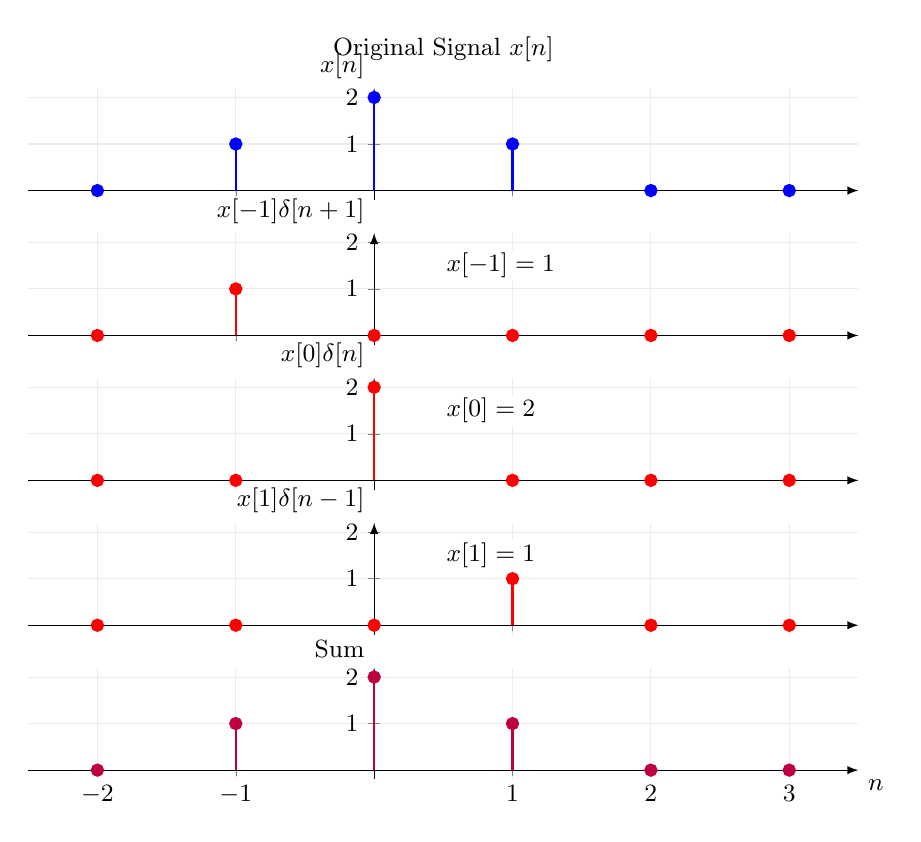
\begin{tikzpicture}
	\begin{groupplot}[
		group style={group size=1 by 5, vertical sep=12pt, xticklabels at=edge bottom},
		/tikz/font=\small,
		width=\linewidth, height=3cm, myaxes,
		xmin=-2.5, xmax=3.5,
		samples at={-2,...,3},
		xtick={-2,-1,0,1,2,3}]
		
		\nextgroupplot[ylabel={$x[n]$}, ymin=-0.2, ymax=2.2, ytick={0,1,2}, title={Original Signal $x[n]$}]
		\addplot[ycomb, mark=*, thick, blue] coordinates {
			(-2,0) (-1,1) (0,2) (1,1) (2,0) (3,0)
		};
		
		\nextgroupplot[ylabel={$x[-1]\delta[n+1]$}, ymin=-0.2, ymax=2.2, ytick={0,1,2}]
		\addplot[ycomb, mark=*, thick, red] coordinates {
			(-2,0) (-1,1) (0,0) (1,0) (2,0) (3,0)
		};
		\node[anchor=west, fill=white, inner sep=1pt] at (axis cs:0.5,1.5) {$x[-1]=1$};
		
		\nextgroupplot[ylabel={$x[0]\delta[n]$}, ymin=-0.2, ymax=2.2, ytick={0,1,2}]
		\addplot[ycomb, mark=*, thick, red] coordinates {
			(-2,0) (-1,0) (0,2) (1,0) (2,0) (3,0)
		};
		\node[anchor=west, fill=white, inner sep=1pt] at (axis cs:0.5,1.5) {$x[0]=2$};
		
		\nextgroupplot[ylabel={$x[1]\delta[n-1]$}, ymin=-0.2, ymax=2.2, ytick={0,1,2}]
		\addplot[ycomb, mark=*, thick, red] coordinates {
			(-2,0) (-1,0) (0,0) (1,1) (2,0) (3,0)
		};
		\node[anchor=west, fill=white, inner sep=1pt] at (axis cs:0.5,1.5) {$x[1]=1$};
		
		\nextgroupplot[xlabel={$n$}, ylabel={Sum}, ymin=-0.2, ymax=2.2, ytick={0,1,2}]
		\addplot[ycomb, mark=*, thick, purple] coordinates {
			(-2,0) (-1,1) (0,2) (1,1) (2,0) (3,0)
		};

	\end{groupplot}
\end{tikzpicture}
		\caption{Signal decomposition using sifting property: $x[n] = \sum_k x[k]\delta[n-k]$.}
		\label{fig:sifting_property_example}
	\end{figure}
	
	\begin{proposition}[General Sifting Property]
		Any discrete-time signal $x[n]$ can be written as:
		\[
		x[n] = \sum_{k=-\infty}^{\infty} x[k]\imp[n-k]
		\]
		
		Similarly, for continuous-time signals:
		\[
		x(t) = \int_{-\infty}^{\infty} x(\tau)\imp(t-\tau) \dd\tau
		\]
	\end{proposition}
	\newpage
	\section*{4.2 The Discrete-Time Convolution Sum}
	
	Now let's see what happens when we put the signal representation into an LTI system $\T$.
	
	\begin{align}
	y[n] &= \T\{x[n]\} = \T\left\{\sum_{k=-\infty}^{\infty} x[k]\imp[n-k]\right\}
	\end{align}
	
	\textbf{Step 1: Use Linearity.} The response to a weighted sum of inputs is the weighted sum of individual responses:
	\[
	y[n] = \sum_{k=-\infty}^{\infty} x[k] \T\{\imp[n-k]\}
	\]
	
	\textbf{Step 2: Use Time-Invariance.} Define the \textbf{impulse response} $h[n] = \T\{\imp[n]\}$. For an LTI system:
	\[
	h_k[n] = \T\{\imp[n-k]\} = h[n-k]
	\]
	

	
	\textbf{Step 3: Combine.} Substituting back gives us the \textbf{discrete-time convolution sum}:
	
	\begin{definition}[Discrete-Time Convolution Sum]
		\[
		y[n] = \sum_{k=-\infty}^{\infty} x[k]h[n-k] = (x \conv h)[n]
		\]
	\end{definition}
	
	\begin{remark}
		The impulse response $h[n]$ completely characterizes the behavior of an LTI system. Given $h[n]$, it is possible to compute the output $y[n]$ for any input $x[n]$. This is \textbf{not} true for nonlinear systems.
	\end{remark}
	
	\begin{figure}[H]
		\centering
		\begin{subfigure}{0.48\textwidth}
	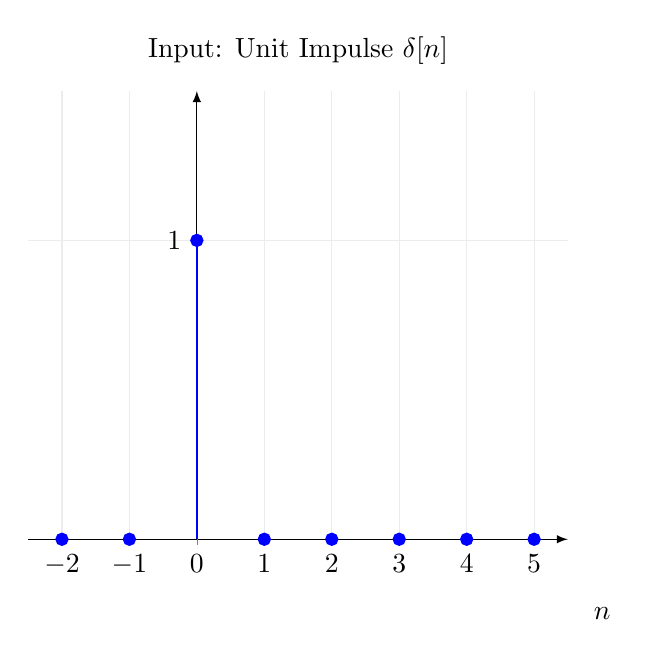
\begin{tikzpicture}
		\begin{axis}[
			myaxes,
			title={Input: Unit Impulse $\delta[n]$}, 
			xlabel={$n$}, ylabel={},
			xmin=-2.5, xmax=5.5, ymin=0, ymax=1.5,
			ycomb,
			xlabel style={at={(axis description cs:1.03,-0.13)}},
			ytick={1}, yticklabels={1},
			xtick={-2,-1,0,1,2,3,4,5},
			extra x ticks={0},
			extra x tick labels={0},
			extra x tick style={grid=none}
			]
			\addplot[blue, thick, mark=*] coordinates {
				(-2,0) (-1,0) (0,1) (1,0) (2,0) (3,0) (4,0) (5,0)
			};
		\end{axis}
	\end{tikzpicture}
\end{subfigure}
\hfill
\begin{subfigure}{0.48\textwidth}
	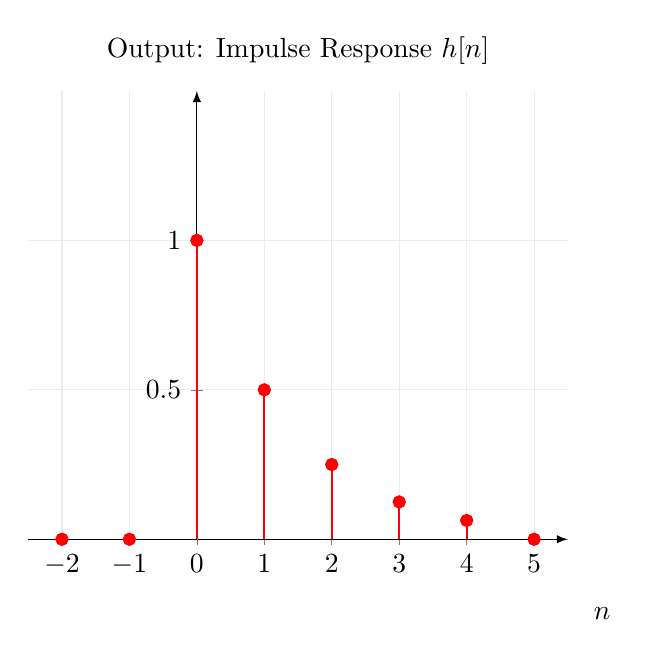
\begin{tikzpicture}
		\begin{axis}[
			myaxes,
			title={Output: Impulse Response $h[n]$}, 
			xlabel={$n$}, ylabel={},
			xmin=-2.5, xmax=5.5, ymin=0, ymax=1.5,
			ycomb,
			xlabel style={at={(axis description cs:1.03,-0.13)}},
			ytick={0.5,1}, yticklabels={0.5,1},
			xtick={-2,-1,0,1,2,3,4,5},
			extra x ticks={0},
			extra x tick labels={0},
			extra x tick style={grid=none}
			]
			\addplot[red, thick, mark=*] coordinates {
				(-2,0) (-1,0) (0,1) (1,0.5) (2,0.25) (3,0.125) (4,0.063) (5,0)
			};
		\end{axis}
	\end{tikzpicture}
\end{subfigure}

		\caption{Impulse response characterizes LTI system completely.}
		\label{fig:impulse_response}
	\end{figure}
	\newpage
\section*{4.3 Examples}

	\paragraph{Convolution as Echo:} 
	Imagine $h[n]$ as an echo pattern. For example, $h[n] = \{1, 0, 0, 0.5, 0, 0.2\}$ models original sound plus delayed echoes.
	
	\paragraph{Convolution as Smoothing:} 
	The impulse response $h[n] = \frac{1}{5}\{1, 1, 1, 1, 1\}$ represents a 5-point moving average filter.
	
	\begin{figure}[H]
		\centering
		\begin{subfigure}{0.48\textwidth}
	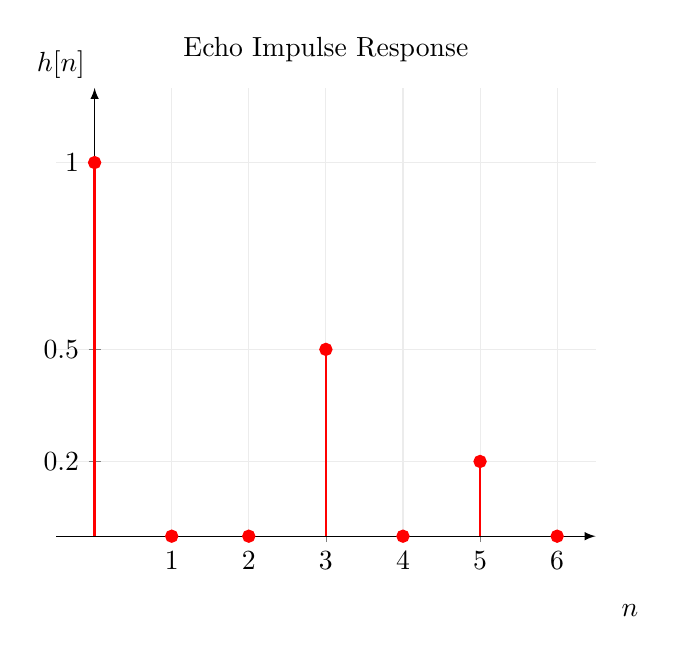
\begin{tikzpicture}
		\begin{axis}[
			myaxes,
			title={Echo Impulse Response}, 
			xlabel={$n$}, ylabel={$h[n]$},
			xmin=-0.5, xmax=6.5, ymin=0, ymax=1.2,
			ycomb,
			xlabel style={at={(axis description cs:1.03,-0.13)}},
			ytick={0.2,0.5,1}, yticklabels={0.2,0.5,1},
			xtick={0,1,2,3,4,5,6},
			]
			\addplot[red, thick, mark=*] coordinates {
				(0,1) (1,0) (2,0) (3,0.5) (4,0) (5,0.2) (6,0)
			};
		\end{axis}
	\end{tikzpicture}
\end{subfigure}
\hfill
\begin{subfigure}{0.48\textwidth}
	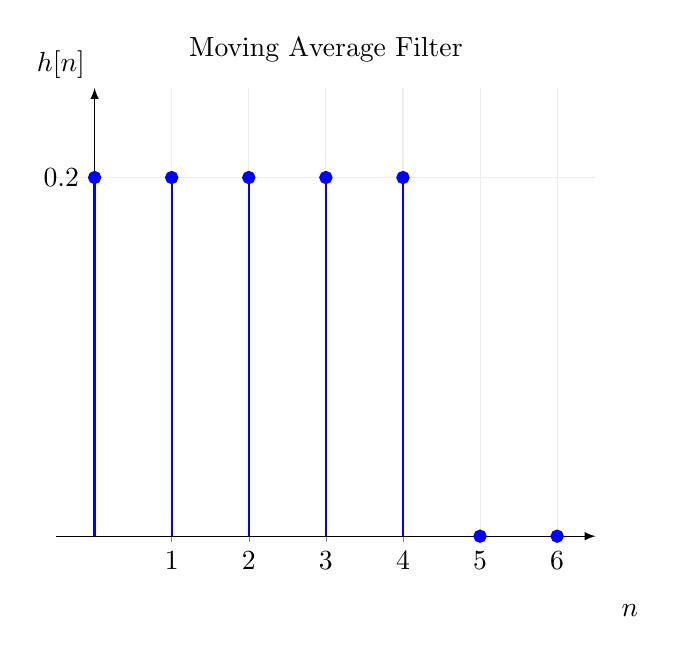
\begin{tikzpicture}
		\begin{axis}[
			myaxes,
			title={Moving Average Filter}, 
			xlabel={$n$}, ylabel={$h[n]$},
			xmin=-0.5, xmax=6.5, ymin=0, ymax=0.25,
			ycomb,
			xlabel style={at={(axis description cs:1.03,-0.13)}},
			ytick={0.2}, yticklabels={0.2},
			xtick={0,1,2,3,4,5,6},
			]
			\addplot[blue, thick, mark=*] coordinates {
				(0,0.2) (1,0.2) (2,0.2) (3,0.2) (4,0.2) (5,0) (6,0)
			};
		\end{axis}
	\end{tikzpicture}
\end{subfigure}

		\caption{Echo system and moving average filter examples.}
		\label{fig:echo_system}
	\end{figure}
	
	\section*{4.4 Computing Convolution: Flip-and-Slide Method}
	
	To compute convolution at a point $n$:
	
	\begin{enumerate}[noitemsep]
		\item \textbf{Plot signals} $x[k]$ and $h[k]$ as functions of dummy variable $k$.
		\item \textbf{Flip} $h[k]$ around zero to get $h[-k]$.
		\item \textbf{Slide} $h[-k]$ by $n$ to obtain $h[n-k]$.
		\item \textbf{Multiply} pointwise: $x[k] \times h[n-k]$.
		\item \textbf{Sum} all products over $k$.
	\end{enumerate}
	\newpage
	\subsection*{4.4.1 Numerical Examples}
	
	\begin{example}[Exponential Input with Unit Step Response]
		Given:
		\[
		x[n] = \left(\frac{1}{2}\right)^{n-1} u[n-1], \qquad h[n] = u[n]
		\]
		
		Find $y[n] = (x \conv h)[n]$.
		
		\textbf{Solution:}
		\begin{align}
		y[n] &= \sum_{k=-\infty}^{\infty} x[k] h[n-k] = \sum_{k=-\infty}^{\infty} \left(\frac{1}{2}\right)^{k-1} u[k-1] \cdot u[n-k]
		\end{align}
		
		For $n < 1$: No overlap, so $y[n] = 0$.
		
		For $n \geq 1$: The sum runs from $k = 1$ to $k = n$:
		\begin{align}
		y[n] &= \sum_{k=1}^{n} \left(\frac{1}{2}\right)^{k-1} = \sum_{r=0}^{n-1} \left(\frac{1}{2}\right)^{r} = \frac{1-(\frac{1}{2})^n}{1-\frac{1}{2}} = 2\left(1-\left(\frac{1}{2}\right)^n\right)
		\end{align}
		
		Therefore: $y[n] = 2\left(1-\left(\frac{1}{2}\right)^n\right) u[n-1]$
	\end{example}
	
	\begin{figure}[H]
		\centering
		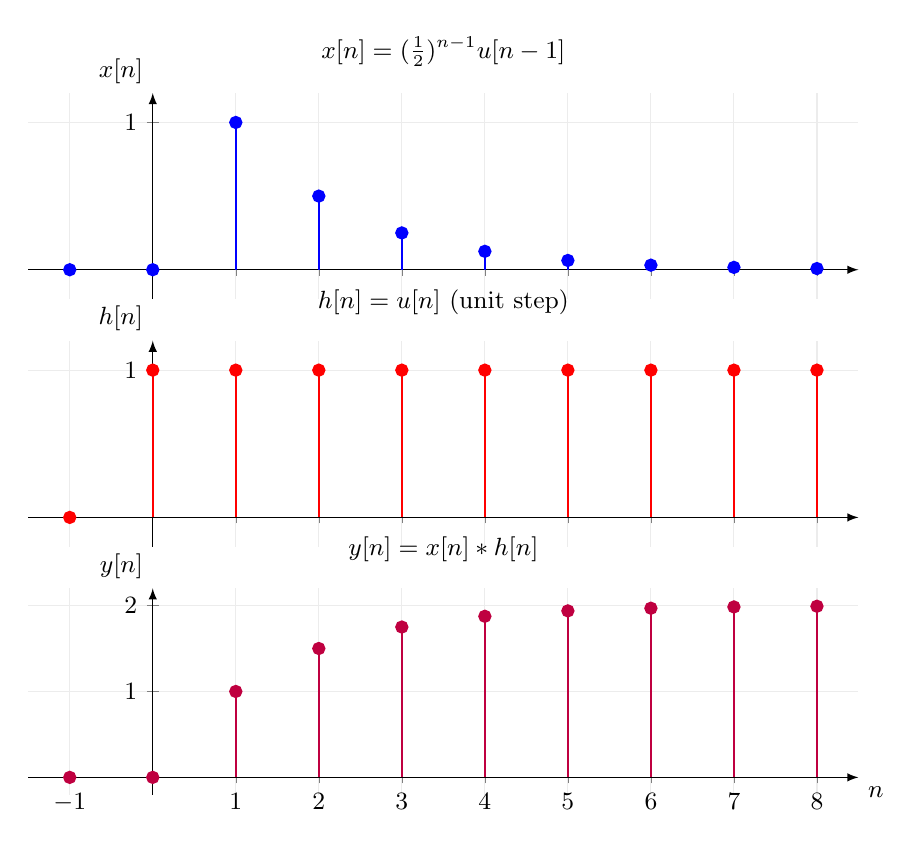
\begin{tikzpicture}
	\begin{groupplot}[
		group style={group size=1 by 3, vertical sep=15pt, xticklabels at=edge bottom},
		/tikz/font=\small,
		width=\linewidth, height=4.2cm, myaxes,
		xmin=-1.5, xmax=8.5,
		samples at={-1,...,8},
		xtick={-1,0,1,2,3,4,5,6,7,8}]
		
		\nextgroupplot[ylabel={$x[n]$}, ymin=-0.2, ymax=1.2, ytick={0,1}, title={$x[n] = (\frac{1}{2})^{n-1}u[n-1]$}]
		\addplot[ycomb, mark=*, thick, blue] coordinates {
			(-1,0) (0,0) (1,1) (2,0.5) (3,0.25) (4,0.125) (5,0.063) (6,0.031) (7,0.016) (8,0.008)
		};
		
		\nextgroupplot[ylabel={$h[n]$}, ymin=-0.2, ymax=1.2, ytick={0,1}, title={$h[n] = u[n]$ (unit step)}]
		\addplot[ycomb, mark=*, thick, red] coordinates {
			(-1,0) (0,1) (1,1) (2,1) (3,1) (4,1) (5,1) (6,1) (7,1) (8,1)
		};
		
		\nextgroupplot[xlabel={$n$}, ylabel={$y[n]$}, ymin=-0.2, ymax=2.2, ytick={0,1,2}, title={$y[n] = x[n] * h[n]$}]
		\addplot[ycomb, mark=*, thick, purple] coordinates {
			(-1,0) (0,0) (1,1) (2,1.5) (3,1.75) (4,1.875) (5,1.938) (6,1.969) (7,1.984) (8,1.992)
		};
	\end{groupplot}
\end{tikzpicture}
		\caption{Exponential decay convolved with unit step.}
		\label{fig:convolution_example1}
	\end{figure}
	\newpage
	\begin{example}[Finite Impulse Response System]
		Consider an LTI system with impulse response:
		\[
		h[n] = \begin{cases}
		2 & n = 0 \\
		-1 & n = 1 \\
		0 & \text{otherwise}
		\end{cases}
		\]
		
		Determine the output for input:
		\[
		x[n] = \begin{cases}
		1 & n = -1 \\
		2 & n = 0 \\
		-1 & n = 1 \\
		0 & \text{otherwise}
		\end{cases}
		\]
		
		\textbf{Solution using the representation:}
		\[
		x[n] = \imp[n+1] + 2\imp[n] - \imp[n-1]
		\]
		
		Since $y[n] = x[n] \conv h[n]$, by linearity:
		\[
		y[n] = h[n+1] + 2h[n] - h[n-1]
		\]
		
		Computing each term:
		\begin{itemize}[noitemsep]
			\item $y[-1] = h[0] = 2$
			\item $y[0] = h[1] + 2h[0] = -1 + 4 = 3$  
			\item $y[1] = h[2] + 2h[1] - h[0] = 0 + 2(-1) - 2 = -4$
			\item $y[2] = h[3] + 2h[2] - h[1] = 0 + 2(0) - (-1) = 1$
			\item $y[3] = h[4] + 2h[3] - h[2] = 0 + 0 - 0 = 0$
			\item $y[n] = 0$ for $n < -1$ or $n > 3$
		\end{itemize}
	\end{example}
	
	\begin{example}[Complex Interval Analysis]
		Let:
		\[
		x[n] = 2\{u[n+2] - u[n-12]\}, \qquad h[n] = \alpha^n\{u[n-2] - u[n-13]\}
		\]
		
		The convolution requires careful interval analysis. The non-zero intervals are:
		\begin{itemize}[noitemsep]
			\item $x[n] \neq 0$ for $-2 \leq n \leq 11$
			\item $h[n] \neq 0$ for $2 \leq n \leq 12$
		\end{itemize}
		
		This leads to five distinct intervals for the output, each requiring separate analysis of the convolution sum limits.
	\end{example}
	
	\section*{Summary and Next Lecture}
	\begin{itemize}[noitemsep]
		\item Any discrete-time signal can be represented as a sum of scaled and shifted impulses: $x[n] = \sum_k x[k]\imp[n-k]$.
		\item The output of a discrete-time LTI system is the convolution sum: $y[n] = \sum_{k=-\infty}^\infty x[k] h[n-k]$.
		\item The impulse response $h[n]$ completely characterizes any LTI system.
		\item Convolution can be computed using the flip-and-slide method or by careful interval analysis.
		\item \textbf{Next time:} Continuous-time convolution integral and properties of convolution.
	\end{itemize}
	
\end{document}